%\textit{All code for simulation can be accessed from GitHub through this link:}

The entire model and simulation code can be found here on \url{https://github.com/kiatvonj/dynein_walk}, where the model and simulation were coded using both Python and C++. The both bound Monte Carlo was coded on Python due to the calculations being less computationally rigorous and time independent, while the one bound Brownian dynamics was coded on C++ to utilize the faster computation speed for the time  dependent Brownian motion.

\section{Simulation}
%\textit{Picking Random angles to create random distribution of dynein configurations. Make sure to clarify that the simulation is split into two parts, the monte carlo both bound and brownian one bound. It is done this way in order for MC to generate ensemble of data rather quickly.}\\
%\textit{Include a flow chart.}
Since we want to generate an ensemble of steps, we use the Monte Carlo method to simulate a single step at a time, as opposed to a walk. This allows us to simplify the code into two respective parts (the Monte Carlo both bound and the Brownian dynamics one bound) that cycles repeatedly after the model takes a step. The simulation starts in the both bound state, where the Monte Carlo randomly picks a both bound configuration and calculate the total energy. If the configuration successfully unbinds, then we use the positions of the domains as initial conditions for the one bound simulation and execute the Brownian dynamics. Once the one bound dynein diffuses onto the microtubule and rebinds, the simulation repeats the cycle and generates a completely different both bound configuration for another step. However, the big caveat with this method is that we must initialize the distance between the binding domains, $L$, in order to ensure that our ensemble covers the whole sample space of possible both bound configurations. This will force the measured probabilities to be a function of $L$ and will be addressed later in Section (\ref{sec:DataAna}). The algorithm for the both bound process is shown below:

\begin{algorithm}[H]
	\caption{Monte Carlo Both Bound}
	\label{alg:MonteCarlo}

	\begin{alg}
	\item Initialize an unsigned distance, $L$, between the binding domains.
	
	\item Randomly pick 4 angles ($\theta_0$, $\theta_1$, $\theta_2$, $\theta_3$) to generate a completely random configuration of dynein in space. (\textit{Include picture})
	
	\item Calculate the distance between the binding domains and check if the distance is within a range of $L\pm l$, where $l$ is arbitrarily small.
	
	\item Rotate the configuration so that both binding domains are on the microtubule and recalculate angles with the naming convention in Figure (\ref{fig:OBvsBB}).
	
	\item Calculate the total energy of the configuration by summing the energy of each domain (using Equation (\ref{eqn:energy})),
	\begin{equation}
		E_{total, i}=\sum_{k}\frac{1}{2}c_k(\theta_k-\theta_{k,eq})^2.
	\end{equation}
	Here, $i$ refers to the specific both bound configuration and $k$ is the domain.	
	
	\item Calculate the relative unbinding probability from a Boltzmann distribution and add a term to the partition function:
	\begin{equation}
		P_{ub} \propto \rho_{ub}e^{-\beta E_{total, n}}\kappa,
	\end{equation}
	\begin{equation}
		Z=\sum_{n}e^{\beta E_{total, n}}.
	\end{equation}
	We defined a $\kappa$ to normalize the relative unbinding probability and keep it less than 1. 
	
	\item ``Roll a die" for a value within the range of $[0,1]$ and check if the value is less than $P_{ub}$. If not, repeat algorithm from step 2.
	
	\item If dynein unbinds, initialize the one bound state with the both bound configuration, run the Brownian dynamics simulation of the step, and wait until it rebinds.
	
	\item Collect statistics about final displacement and one bound time. Repeat algorithm from step 2. 
	
	\end{alg}

\end{algorithm}

A more in-depth explanation and rigorous flow chart for the one bound Brownian dynamics simulation can be found here \cite{Capek2017, }.

%\section{Time Evolution}
%\textit{Simulate over a delta t during one bound and every iteration check for rebinding. How are the probabilities of binding and unbinding affected by the time.}

\section{Constants}
\textit{How we defined our constants based on experiment and pictures.  Need to include figures here of experiment dynein and how we measure the pre and post stroke equilibrium angles.}

\begin{figure}[hbt!]
	\centering
	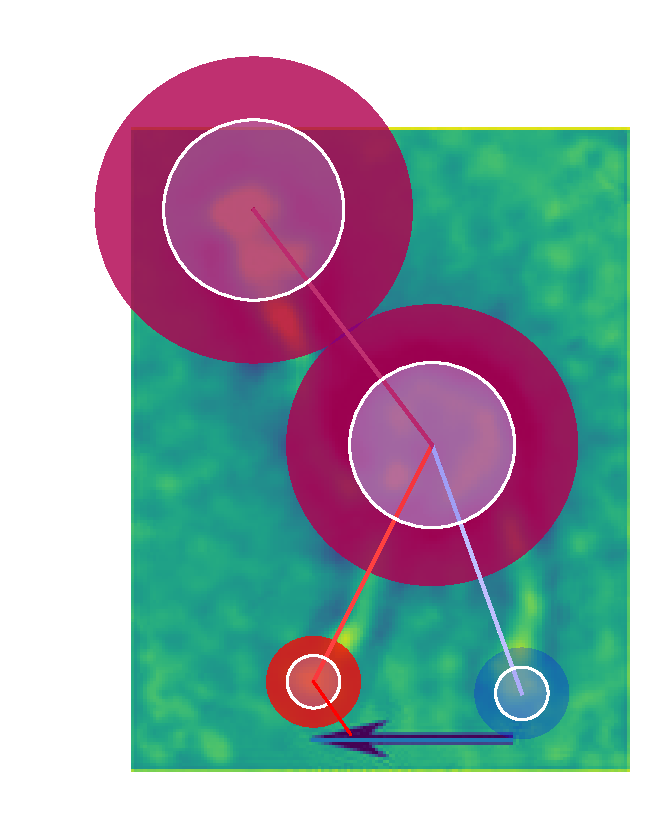
\includegraphics[width=0.3\columnwidth]{../../plots/burgess-model-figure.pdf}
	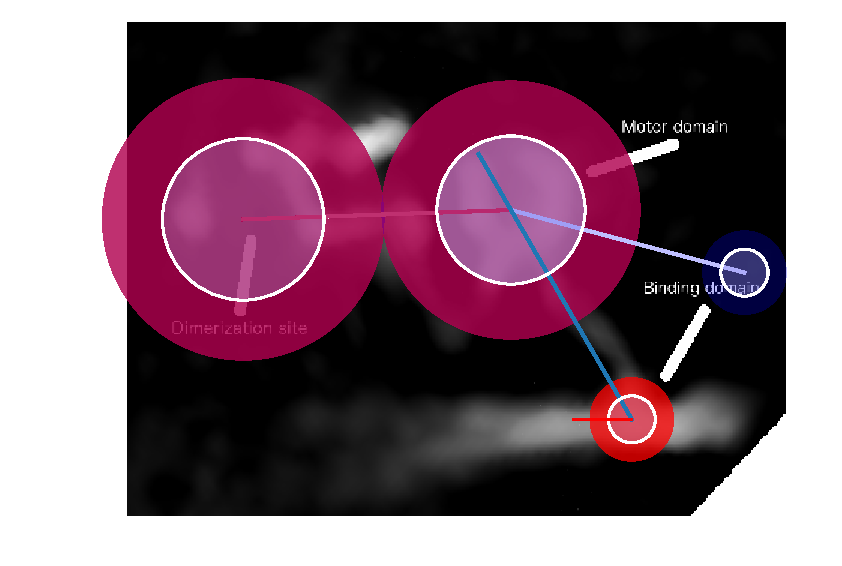
\includegraphics[width=0.5\columnwidth]{../../plots/grotjahn-model-figure.pdf}%
	\caption[Experimental Pictures of Dynein for Model Parameters]{\textbf{Experimental Pictures of Dynein for Model Parameters} Left: the both bound model is superimposed over dynein micrograph. The arrow indicates 15nm. Image taken from \cite{burgess2003dynein}.  Right: cryo-electron tomograph of dynein with the one-bound model overlaid. Image taken from \cite{grotjahn}.} 
	\label{fig:ModelParams}
\end{figure}


\section{Parameter Fitting}
\textit{How we will fit our parameters to agree with Yildiz' experimental data of dynein stepping.}

\subsection{Rate Constants}
\textit{Fitting our rate constants were a huge part of our model and how we made sure our dynein can match experimentalist results.}

\section{Model Validation}
\textit{Any tests of our model to make sure the code is reasonably sound and that the physics makes sense. Make sure there is no bugs in code. What was the bug testing procedure.}

\section{Data Analysis} \label{sec:DataAna}
\begin{equation}
	p(x_i,x_f)=p(x_f|x_i)p(x_i)
\end{equation}
Bayes' Theorem
\begin{equation}
	p(x_i|L_i)=\frac{p(L_i|x_i)p(x_i)}{p(L_i)}
\end{equation}
\[
	p(x_i|L_i)=\frac{p(x_i)}{p(L_i)} 
\]\[
	p(x_i)=p(x_i|L_i)p(L_i)
\]
Detailed Balance Equation:
\begin{equation}
	p^n(L_i)=T^n(L_f|L_i)p^0(L_i)
\end{equation}
\begin{align}
	T(L_f|L_i)&=I(L_f|x_i)p(x_f|x_i)p(x_i|L_i)\\
	&=p(L_f|x_i)p(x_i|L_i)\\
	&=p(L_f|L_i)
\end{align}



